\documentclass{standalone}
\usepackage{tikz}
\usetikzlibrary{angles,quotes}
\begin{document}
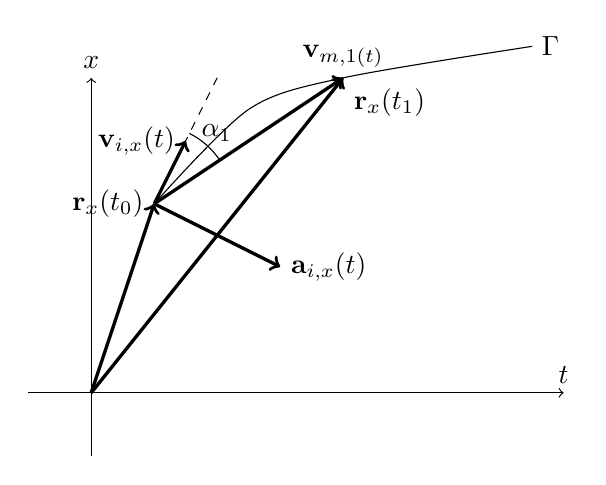
\begin{tikzpicture}[scale = 4]
    \coordinate (O) at (0,0);
    \draw[->] (-0.2, 0) -- (1.5, 0) coordinate (t) node[above]{$t$};
    \draw[->] (0,-0.2) --(0,1) coordinate (x) node[above]{$x$};
    \draw[->,very thick] (O) -- (0.2, 0.6) node[left] {$\mathbf{r}_x(t_0)$};
    \draw[dashed] (0.2, 0.6) coordinate (r) -- (0.4, 1) coordinate (rx);
    \draw[->,very thick] (O) -- (0.8, 1) coordinate (r2) node[below right] {$\mathbf{r}_x(t_1)$};
    
    \draw[->,very thick] (0.2, 0.6) -- (0.3, 0.8) node[left] {$\mathbf{v}_{i,x}(t)$};
    \draw[->,very thick] (0.2, 0.6) -- (0.8, 1) node[above] {$\mathbf{v}_{m,1(t)}$};
    
    \draw[->,very thick] (0.2, 0.6) -- (0.6,0.4) node[right] {$\mathbf{a}_{i,x}(t)$};

    \draw[-,thin] plot [smooth] coordinates {(0.2, 0.6) (0.5, 0.9) (0.8, 1) (1.4, 1.1)} node[right] {$\Gamma$};
    
    \pic["$\alpha_1$", draw=black, -, angle eccentricity=1.2, angle radius=1cm] {angle=r2--r--rx};
\end{tikzpicture}
\end{document}